\documentclass[13pt,aspectratio=169,t,xcolor=table]{beamer}
\usepackage[utf8]{inputenc}

\usepackage{booktabs} 
\usepackage{subcaption}
\usepackage{adjustbox}

\usetheme{Ufg}

%-------------------------------------theorems--------------
\newtheorem{conj}{Conjetura}
\newtheorem{defi}{Definição}
\newtheorem{teo}{Teorema}
\newtheorem{lema}{Lema}
\newtheorem{prop}{Proposição}
\newtheorem{cor}{Corolário}
\newtheorem{ex}{Exemplo}
\newtheorem{exer}{Exercício}

\setbeamertemplate{theorems}[numbered]
\setbeamertemplate{caption}[numbered]

%-------------------------------------------------------------%
%----------------------- Primary Definitions -----------------%

% This command set the default Color, is also possible to choose a custom color
\setPrimaryColor{TorVergataGreen} 

% First one is logo in title slide (we recommend use a horizontal image), and second one is the logo used in the remaining slides (we recommend use a square image)
\setLogos{lib/logos/LOGO-ATENEO_BIANCO_20230308.png}{lib/logos/LOGO-ATENEO_Variante1_Bianco_20230307.png} 


% -------------------------------------- Title Slide Information
\begin{document}
\title[Inf UFG]{Hard Disk Failure Data Processing}
\subtitle{Corso di Sistemi ed Architetture per Big Data}

\author{
    \begin{tabular}{c c}
    Luca Falasca & Matteo Conti \\
    0334722 & 0323728
  \end{tabular}
}

\institute[UFG] % (optional)
{
  Progetto 1 - Batch processing
}
\date{2024}
%-----------------------The next statement creates the title page.
\frame[noframenumbering]{\titlepage}


%------------------------------------------------Slide 1
\setLayout{vertical} % This command define the layout. 'vertical' can be replace with 'horizontal', 'blank, 'mainpoint', 'titlepage'

\begin{frame}
    \frametitle{Indice}
    \tableofcontents
\end{frame}
%---------------------------------------------------------


%---------------------INTRODUZIONE---------------------------
%---------------------------------------------------------Slide 2
\setLayout{mainpoint}
\setBGColor{TorVergataGreen}
\begin{frame}{}
    \frametitle{Introduzione}
\end{frame}
%---------------------------------------------------------

\section{Introduzione}
\subsection{Obbiettivi}
%---------------------------------------------------------Slide 3
\setLayout{vertical}
\begin{frame}{Introduzione-Obbiettivi}
    Il progetto verte sull'analisi di un dataset contenente dati riguardanti il monitoraggio di dischi rigidi installati all'interno di un cluster di server gestito da un cloud provider, in particolare si vuole: 
    \vspace{0.3cm}
    \begin{itemize}
        \item Realizzare una pipeline di elaborazione dati
        \item Eseguire le query richieste dalla specifica
        \item Visualizzare i risultati
        \item Analizzare le performance ottenute con i formati dati CSV e Parquet
    \end{itemize}
    \vspace{0.3cm}
    \begin{figure}
        \raggedright
        \hspace{2cm}
        
\includegraphics[width=.7\textwidth]{res/intro_icon.png}
    \end{figure}
\end{frame}
%---------------------------------------------------------

%---------------------------------------------------------Slide 4
\subsection{Dataset}
\setLayout{vertical}
\begin{frame}{Introduzione-Dataset}
    Il dataset fornito è una versione ridotta di quello presentato nel Grand Challenge della conferenza ACM DEBS 2024. Delle numerose colonne presenti nel dataset, ne verranno selezionate
    solamente cinque, in particolare:
    \begin{itemize}
        \item \textit{date}: data della misurazione nel formato 'YYYY-MM-DD'
        \item \textit{serial\_number}: identificativo del disco rigido
        \item \textit{model}: modello del disco rigido
        \item \textit{s9\_power\_on\_hours}: tempo di accensione del disco rigido in ore
        \item \textit{vault\_id}: identificativo del gruppo di storage server a cui il disco rigido appartiene
        \item \textit{failure}: flag che indica se il disco rigido ha subito una failure o meno
    \end{itemize}
\end{frame}
%---------------------------------------------------------

%---------------------PIPELINE---------------------------
%---------------------------------------------------------Slide 5

\setLayout{mainpoint}
\setBGColor{TorVergataGreen}
\begin{frame}{}
    \frametitle{Pipeline}
\end{frame}
%---------------------------------------------------------

\section{Pipeline}
%---------------------------------------------------------Slide 6
\setLayout{vertical}
\begin{frame}{Pipeline}
    La pipeline di elaborazione dati è stata containerizzata e deployata tramite docker compose ed è composta da cinque componenti:
    \begin{itemize}
        \item Data ingestion
        \item Data storage
        \item Data processing
        \item Analytical data storage
        \item Data visualization
    \end{itemize}
    \begin{adjustbox}{margin=0.5cm 0cm 0cm 0.58cm, center} % left, bottom, right, top 
        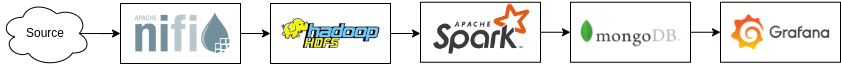
\includegraphics[width=.99\textwidth]{res/pipeline.png}
    \end{adjustbox}
\end{frame}
%---------------------------------------------------------
\subsection{Data ingestion}
%---------------------------------------------------------Slide 7
\begin{frame}{Pipeline - Data ingestion}
    Per la data ingestion è stato utilizzato il framework Apache NiFi, il quale si occupa di:
    \begin{columns}
        \column{0.5\textwidth}
            \begin{minipage}[b]{1\textwidth}
                \begin{itemize}
                    \item Ricevere tramite HTTP il file CSV contenente i dati
                    \item Filtrare i dati
                    \item Memorizzare i dati su HDFS in formato Parquet e CSV
                \end{itemize}
            \end{minipage}
        \column{0.5\textwidth}
            \begin{minipage}{1\textwidth}
                \begin{adjustbox}{margin=0cm 0cm 1.7cm 0cm, center} % left, bottom, right, top
                    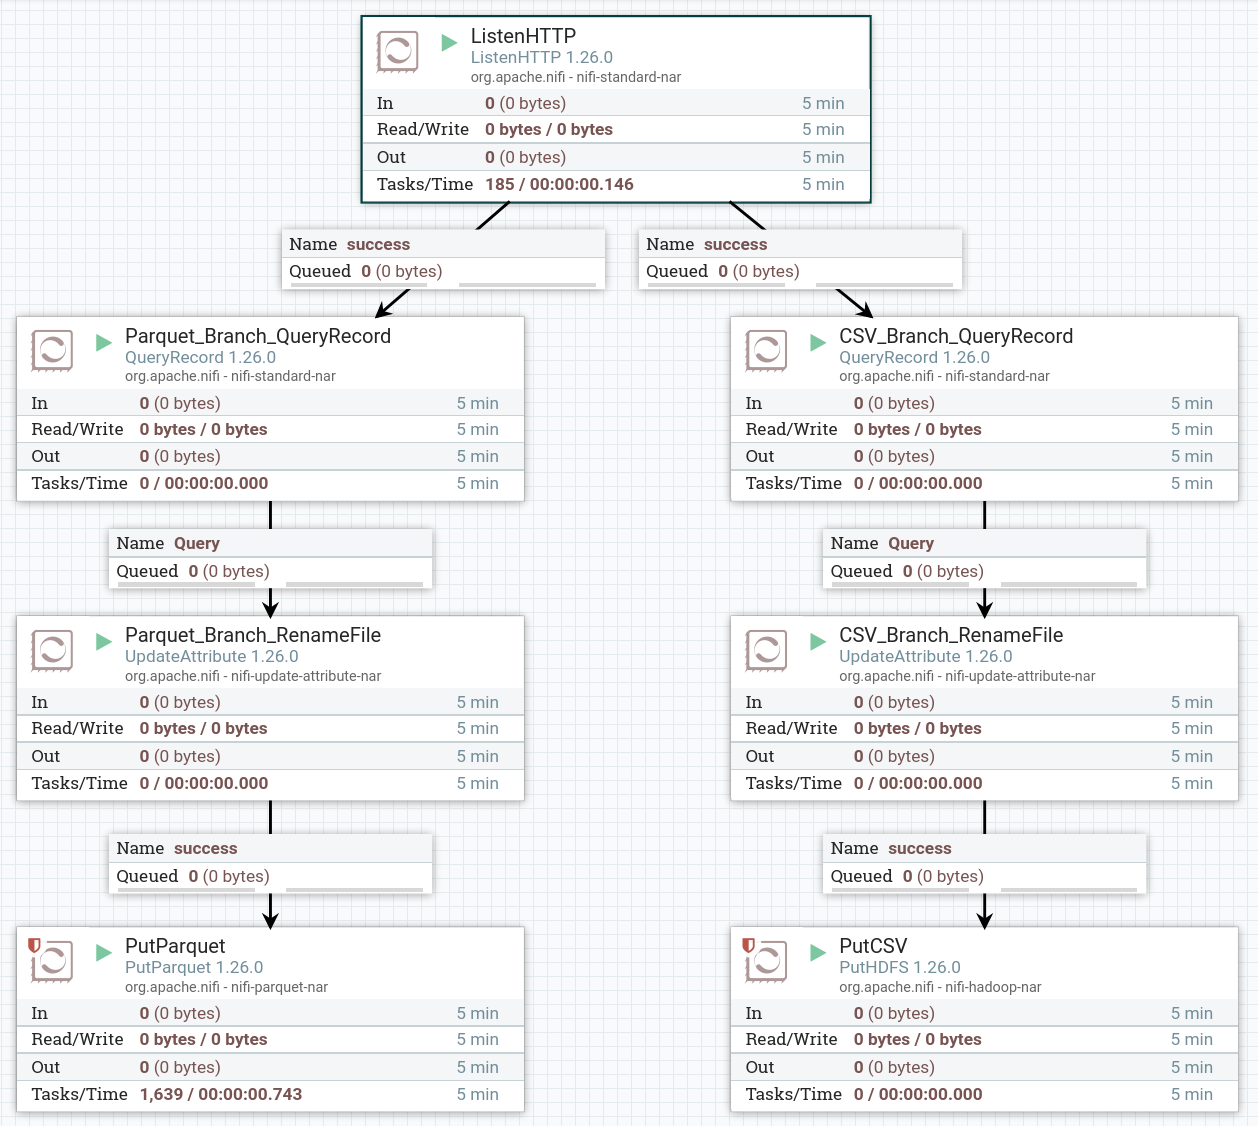
\includegraphics[width=1\textwidth]{res/nifi_flow.png}
                \end{adjustbox}
            \end{minipage}
    \end{columns}
\end{frame}
%---------------------------------------------------------
\subsection{Data storage}
\subsection{Data processing}
\subsection{Analytical data storage}
\subsection{Data visualization}

%---------------------CONCLUSIONI---------------------------
\setLayout{mainpoint}
\setBGColor{TorVergataGreen}
\begin{frame}{}
    \frametitle{Conclusione}
\end{frame}
\section{Conclusioni}
\subsection{Performance}

%--------------------------------------------------------- Slide 5
\section{Changing colors and Layouts}

\setLayout{blank} % Example of changing layout
\setBGColor{DarkOrange}  %Example of changing background color 

\begin{frame}{Clean layout and two-column text}
    
    \begin{columns}
    
        \column{0.5\textwidth}
        This is a text in first column.
        $$E=mc^2$$
        $$ 1 + 2 + \cdots + k =  \frac{k \cdot (k + 1)}{2}.$$
        \begin{itemize}
        \item First item
       
        \item Second item
        \end{itemize}
        
        \column{0.5\textwidth}
        This text will be in the second column
        and on a second tought this is a nice looking
        layout in some cases.
        
        \begin{enumerate}
            \item First
            \item Second
        \end{enumerate}
        
    \end{columns}
    
\end{frame}
%---------------------------------------------------------


%---------------------------------------------------------Slide 6
%Highlighting text
\setLayout{vertical}
\begin{frame}{Sample frame title}
    
    In this slide, some important text will be
    \alert{highlighted} because it's important. Please, don't abuse it.
    
    \begin{block}{Remark}
        Sample text
    \end{block}
    
    \begin{alertblock}{Important theorem}
        Sample text in alert box
    \end{alertblock}
    
    \begin{examples}
        Sample text in green box. The title of the block is ``Examples".
    \end{examples}
    
\end{frame}
%---------------------------------------------------------


%---------------------------------------------------------Slide 7


\setLayout{mainpoint}
\setBGColor{DarkPurple}
\begin{frame}{}
    \frametitle{Preliminary Empirical Study}
\end{frame}
%-------------------------------------------------------


%---------------------------------------------------------Slide 8

\setLayout{horizontal}
\begin{frame}
    \frametitle{Sample frame title}
    This is a text in second frame. For the sake of showing an example.
    
    \begin{itemize}
        \item<1-> Text visible on slide 1
        \item<2-> Text visible on slide 2
        \begin{itemize}
            \item text subitem
        \end{itemize}
        \item<3> Text visible on slides 3
        \item<4-> Text visible on slide 4
    \end{itemize}
\end{frame}
%---------------------------------------------------------

%---------------------------------------------------------Slide 10
\setLayout{titlepage}
\setBGColor{DarkGray}
\titlepage
%-------------------------------------

\end{document}